\chapter{Sensitivitätsanalyse}\label{ch:Sensitivity}
In diesem Kapitel wird das in Kapitel \ref{ch:ch2} hergeleitete lineare Modell des Antriebsstrangs auf die Sensitivität verschiedener Parameter und Eingänge untersucht. Damit soll die Relevanz für eine Parameter- und Eingangsschätzung im folgenden Kapitel belegt und unterstrichen werden.
Eine mögliche Definition für eine Sensitivitätsanalyse ist die folgende: \emph{The study of how uncertainty in the output of a model (numerical or otherwise) can be apportioned to different sources of uncertainty in the model input} \cite{Saltelli.2004}.
Für die Analyse gibt es verschiedene Methoden. Dabei ist die OAT(one-at-a-time)-Methode wohl die einfachste. Dabei wird pro Simulationsdurchlauf lediglich eine Eingangsgröße geändert während alle anderen auf den nominal Werten gehalten werden. Die Methode liefert aber nur eine sehr beschränkte Aussage über den gesamten Eingangsraum. Jedoch kann sie für die Abschätzung einer ersten Untergruppe an relevanten Eingängen hilfreich sein.    

 Die in der Literatur am häufigsten diskutierten Ansätze basieren auf partiellen Ableitungen der Art $\partial y_i/\partial x_i$ wobei $y$ ein beliebiger Ausgang und $x_i$ ein beliebiger Eingang des Systems ist. Ein Eingang kann hierbei auch ein variierender Parameter sein. Dieses Vorgehen wird vor allem bei relativ einfachen, mathematisch wohlbestimmten und stetigen Modellen verwendet. Der Vorteil dabei ist, dass die Sensitvitätsfunktionen sobald sie einmal berechnet sind leicht an Veränderungen anpassbar sind und auch für ähnliche Systeme verwendet werden können \cite{Karnavas.1993}. Jedoch werden die partiellen Ableitung immer in einem bestimmen Arbeitspunkt berechnet d.h. die Aussagen der Sensitvitätsfunktionen gelten für nichtlineare Systeme nur lokal um diesen den Arbeitspunkt. Des weiteren ist es oft sehr schwer oder gar unmöglich die benötigten Ableitungen für komplexe Modelle zu berechnen.

Eine Alternative zur Berechnung der partiellen Ableitungen sind globale Methoden. Hierbei werden die Modelleingänge stochstisch varriert, woraus sich nach vielen Simulationen eine Strichprobe für die Modellausgänge ergibt. Dieses Methode der mehrfachen Simulation wird auch Monte-Carlo-Methode genannt. Wie der Name schon sagt ist der grundlegende Vorteil dabei, dass durch eine genügend große Stichprobe eine globale Aussage zur Sensitivität gegeben werden kann. Des weiteren erlaubt die Methode auch Aussagen über die verkoppelte Wirkung von Eingangsänderungen ohne spezielles Vorwissen über die Struktur des Modells. Der entscheidende Nachteil liegt je nach Stichprobengröße und Komplexität des Modells in der Rechenzeit.      

Aufgrund des linearen und stetigen Charakters von \eqref{eq:sys_linex} werden für diese Arbeit die partiellen Ableitungen für die Sensitivitätsanalyse verwendet.
Hierfür wird zuerst ein idealer Schaltvorgang beschrieben um die Sensitivitätsfunktionen in verschieden Schaltphasen auswerten zukönnen. Des weiteren wird mit der Berechnung der Fisher-Informationsmatrix eine Abschätzung für die erreichbare Genauigkeit der Schätzungen geliefert.
   
\section{Beschreibung eines Gangwechsels}\label{sec:Gangwechsel}
Bei einem Gangwechsel wird durch die Betätigung von Schaltelementen die Übersetzung des Getriebes geändert. Dies soll zum Einen in jedem Fall möglichst ohne für den Fahrer spürbare unerwünschte Beschleunigungen am Getriebeabtrieb passieren. Zum Anderen soll der Gangwechsel aber auch so schnell wie möglich und ohne Momentenunterbrechung vollzogen werden. Es besteht also eine Zielkonflikt zwischen den Komfortansprüchen des Fahrers und der Dauer eines Schaltvorgangs. Grundsätzlich wird ein Gangwechsel auf zwei Ebenen unterschieden. Zum einen die Richtung der Übersetzung $i_\mathrm{Gang}$. Bei einer Hochschaltung wird $i_\mathrm{Gang}$ kleiner und entsprechend bei einer Rückschaltung größer. Zum anderen die Richtung der Last am Getriebeeingang. Ist diese positiv spricht man von einer Zugschaltung bei negativem Antriebsmoment von einer Schubschaltung \cite{Fischer.2016}.
In dieser Arbeit werden die Betrachtungen auf eine Zug-Hoch-Schaltung zwischen dem zweitem und dem dritten Gang reduziert. Dies hat zum Einen den Grund, dass in diesen Gängen der Drehmomentenwandler überbrückt und die Trennkupplung geschlossen ist, sodass deren Dynamik vernachlässigt werden kann. Zum Anderen ist dies eine häufige Schaltung im Fahrzeugbetrieb. Die Erkenntnisse können jedoch auch auf andere Gangwechsel übertragen werden.

Bei dem in dieser Arbeit betrachteten Getriebe wird ein Gangwechsel mittels der Schließung und der simultanen Öffnung einer Bremse bzw. Kupplung realisiert. Bei der Schaltung zwischen dem zweiten und dritten Gang sind dies die Bremse $B_\mathrm{05}$ und die Kupplung $K_\mathrm{38}$. Der Gangwechsel wird in die in Abbildung \ref{fig:23zughoch_schema} gezeigten vier Phasen 2. Gang, Momentenübergabe, Drehzahlsynchronisation und 3. Gang eingeteilt.

Im 2. Gang ist die Kupplung $K_\mathrm{38}$ geschlossen und überträgt das volle Antriebsmoment. Die Differenzdrehzahl $\Delta \omega_{38}$ der Wellen 3 und 8 ist somit gleich Null. Die Bremse $B_\mathrm{05}$ ist geöffnet und überträgt kein Drehmoment. Vor dem Gangwechsel wird die Kupplung $K_\mathrm{38}$ durch eine Reduzierung des anliegenden Drucks ins Schleifen gebracht, sodass sich an der Kupplung eine minimale Drehzahldifferenz ergibt. Dadurch wirkt an den Scheiben der Kupplung die Gleitreibung, welche somit der Reaktionskraft an den Kupplungen entspricht. Der Betrag der Geleitreibung kann, wie in \ref{sec:mod_reib} beschrieben, mit dem Reibungskoeffizient und der Normalkraft berechnet werden.

Somit kann während der Momentenübergabe das Drehmoment an $K_\mathrm{38}$ abgesenkt werden, während gleichzeitig $B_\mathrm{05}$ mit Hilfe eine Vorsteuerung derart geschlossenen wird, dass stets das volle Antriebsmoment übertragen wird und $K_\mathrm{38}$ im Schleifen gehalten wird. Die Herleitung einer derartigen Vorsteuerung kann \cite{Weber.2018} entnommen werden.    
  
Wenn $K_\mathrm{38}$ vollständig geöffnet ist d.h. kein Drehmoment mehr übertragen wird beginnt die Drehzahlsynchronisation. Diese kann auf zwei Arten vollzogen werden. Zum einen kann das Drehmoment an $B_\mathrm{05}$ überhöht werden, wodurch die Differenzdrehzahl $\Delta \omega_{05}$ auf Null gebracht wird und die Antriebsdrehzahl abgesenkt wird. Eine weitere Möglichkeit, die sich besonders bei Hybridgetrieben anbietet, ist die Drehzahlsynchronisation mittels einer Absenkung des Antriebsmomentes herzustellen. Mit einer E-Maschine kann die Absetzung schneller und genauer vollzogen werden, als mit einem Verbrennungsmotor. Bei dem in dieser Arbeit betrachteten Gangwechsel werden beide Möglichkeiten gleichzeitig genutzt.

Am Ende der Drehzahlsynchronisation ist $\Delta \omega_{05}=0$ und die Getriebeübersetzung liegt auf dem Niveau des dritten Gangs.

In Abbildung (???) sind die Drehzahlgeschwindigkeiten $\omega_1$, $\omega_2$, $\omega_\mathrm{C}$ und die Verdrehung der Seitenwelle $\phi$ für den in dieser Arbeit verwendeten Gangwechsel zu sehen. Zusätzlich zeigt Abbildung (???) die dazugehörigen Beschleunigungen $\dot{\omega_1}$, $\dot{\omega_2}$, $\dot{\omega_\mathrm{C}}$ und die Verdrehgeschwindigkeit $\dot{\phi}$.

\begin{figure}[t]
	\centering 
	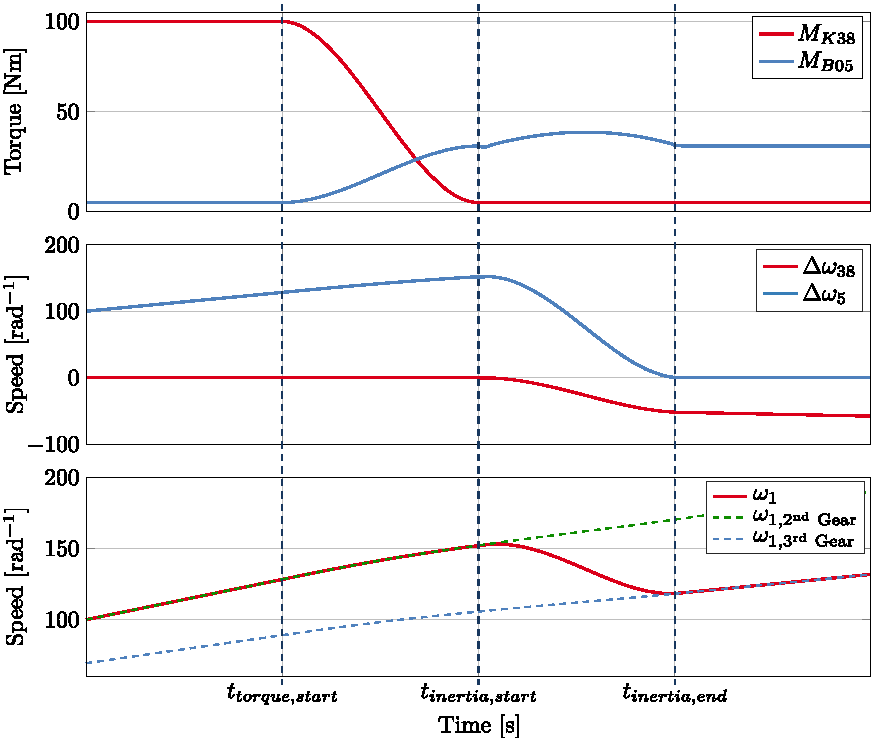
\includegraphics[scale=1]{figures/03_Sensitivitaetsanalyse/01_Gangwechsel/23Shift}
	\caption{Schematische Darstellung des Gangwechsels aus dem zweiten in den dritten Gang.}
	\label{fig:23zughoch_schema} % always use \label AFTER \caption
\end{figure}

\section{Anwendung der Paramater- und Eingangssensitivitätsanalyse}\label{sec:para_sens}
Wie einleitend erläutert werden die Sensitiviäten in dieser Arbeit mittels partiellen Differentialen berechnet. Nach \cite{Hearne.1985} ist für ein nichtlineares System erster Ordnung
\begin{equation}
\mathrm{d} x_i/\mathrm{d} t = f_i(\pmb{x},\pmb{p},\pmb{u})\quad i=1,2,\,\dots\, ,n 
\end{equation}
mit dem Zustandsvektor $\pmb{x} = [x_1, x_2,\, \dots\, ,x_n]^T$, dem Parametervektor $\pmb{p} = [p_1, p_2,\, \dots\, ,p_m]^T$, dem Eingangsvektor $\pmb{u} = [u_1, u_2,\, \dots\, ,p_l]^T$ und der differenzierbaren Funktion $f_i$ die absolute Parametersensitivitätsfunktion definiert als
\begin{equation}\label{eq:abs_psens}
S_{ij} = \partial x_i/\partial p_j \quad i=1,2,\,\dots\, ,n \quad j=1,2,\,\dots\, ,m.
\end{equation}
Die entsprechende normalisierte Parametersensitivitätsfunktion ist 
\begin{equation}
S_{\mathrm{N},ij} = \partial x_i/\partial p_j\ p_{j0}/x_{i0}.
\end{equation}
Die normalisierte Parametersensitivitätsfunktion $S_{ij}$ kann interpretiert werden, als approximierte prozentuale Änderung des Zustandes $x_i$ für eine $1\%$-ige Änderung des Parameters $p_j$. Das Modell des Antriebsstrangs ist mit \eqref{eq:sys_linex} in der Form
\begin{equation}
\dot{\pmb{x}} = \pmb{f}(t,\pmb{x}(t,\pmb{p}),\pmb{p})+ \pmb{B}(\pmb{p})\pmb{u}(t) 
\end{equation} 
gegeben. Wendet man \eqref{eq:abs_psens} auf diese Gleichung an erhält man unter Berücksichtigung der Kettenregel
\begin{equation}\label{eq:Sens_eq}
\mathrm{d} \pmb{S}_j/\mathrm{d} t = \dot{\pmb{S}}_j= \frac{\partial\pmb{f}(t,\pmb{x}(t,\pmb{p}),\pmb{p})}{\partial \pmb{x}}\,\pmb{S}_j+\frac{\partial\pmb{f}(t,\pmb{x}(t,\pmb{p}),\pmb{p})}{\partial \pmb{p}}+\frac{\partial \pmb{B}(\pmb{p})}{\partial \pmb{p}}\,\pmb{u}(t).
\end{equation}
Die Parametersensitivitätsfunktion werden im Folgenden anhand \eqref{eq:sys_nl} für $m_\mathrm{veh}$, $k_\mathrm{ss}$, $d_\mathrm{ss}$, $\mu_{38}$ und $\zeta$ gebildet und die zeitlichen Verläufe von $\pmb{S}$ für einen Schaltvorgang gemäß \ref{sec:Gangwechsel} interpretiert.

\subsection{Sensitivität des Zustandes $\pmb{x}$ von $k_\mathrm{ss}$}
Die Sensitivität von \eqref{eq:sys_ex23lin} vom Parameter $k_\mathrm{ss}$ ergibt sich mit \eqref{eq:Sens_lineq} zu 
\begin{align}
\dot{\pmb{S}}_{k_\mathrm{ss}} &= \begin{bmatrix} 0 & -0,799\, d_\mathrm{ss,0} & -1,97\, k_\mathrm{ss,0} & 1,97\, d_\mathrm{ss,0} \\ 0 & -0,248\, d_\mathrm{ss,0} & -0,612\, k_\mathrm{ss,0} & 0,612\, d_\mathrm{ss,0} \\ 0 & 0,405 & 0 & -1,0 \\ 0 & \frac{0,81\, d_\mathrm{ss,0}}{0,108 \, m_\mathrm{veh,0} + 6,4} & \frac{2,0\, k_\mathrm{ss,0}}{0,108\, m_\mathrm{veh,0} + 6,4} & -\frac{2,0\, d_\mathrm{ss,0}}{0,108\, m_\mathrm{veh,0}+6,4}\end{bmatrix} \pmb{S}_{k_\mathrm{ss}} \\
&+ \begin{bmatrix} 0 & 0 & -1,97 & 0 \\ 0 & 0 & -0,612 & 0 \\ 0 & 0 & 0 & 0 \\ 0 & 0 & \frac{2,0}{0,108\, m_\mathrm{veh,0} + 6,4}  & 0 \end{bmatrix}\pmb{x}_\mathrm{ex}.
\end{align}


\subsection{Sensitivität des Zustandes $\pmb{x}$ von $d_\mathrm{ss}$}
Die Sensitivität von \eqref{eq:sys_ex23lin} vom Parameter $d_\mathrm{ss}$ ergibt sich mit \eqref{eq:Sens_lineq} zu
\begin{align}
\dot{\pmb{S}}_{d_\mathrm{ss}} &= \begin{bmatrix} 0 & -0,799\, d_\mathrm{ss,0} & -1,97\, k_\mathrm{ss,0} & 1,97\, d_\mathrm{ss,0} \\ 0 & -0,248\, d_\mathrm{ss,0} & -0,612\, k_\mathrm{ss,0} & 0,612\, d_\mathrm{ss,0} \\ 0 & 0,405 & 0 & -1,0 \\ 0 & \frac{0,81\, d_\mathrm{ss,0}}{0,108 \, m_\mathrm{veh,0} + 6,4} & \frac{2,0\, k_\mathrm{ss,0}}{0,108\, m_\mathrm{veh,0} + 6,4} & -\frac{2,0\, d_\mathrm{ss,0}}{0,108\, m_\mathrm{veh,0}+6,4}\end{bmatrix} \pmb{S}_{k_\mathrm{ss}}\\ 
&+ \begin{bmatrix} 0 & -0,799 & 0 & 1.973 \\ 0 & -0,248 & 0 & 0,612 \\ 0 & 0 & 0 & 0 \\ 0 & \frac{0,81}{0,108 \, m_\mathrm{veh,0} + 6,4} & 0 & -\frac{2,0}{0,108\, m_\mathrm{veh,0}+6,4} \end{bmatrix}\pmb{x}_\mathrm{ex}.
\end{align}

\subsection{Sensitivität des Zustandes $\pmb{x}$ von $m_\mathrm{veh}$}
Die Sensitivität von \eqref{eq:sys_ex23lin} vom Parameter $m_\mathrm{veh}$ ergibt sich mit \eqref{eq:Sens_lineq} zu
\begin{align}
\dot{\pmb{S}}_{m_\mathrm{veh}} &= \begin{bmatrix} 0 & -0,799\, d_\mathrm{ss,0} & -1,97\, k_\mathrm{ss,0} & 1,97\, d_\mathrm{ss,0} \\ 0 & -0,248\, d_\mathrm{ss,0} & -0,612\, k_\mathrm{ss,0} & 0,612\, d_\mathrm{ss,0} \\ 0 & 0,405 & 0 & -1,0 \\ 0 & \frac{0,81\, d_\mathrm{ss,0}}{0,108 \, m_\mathrm{veh,0} + 6,4} & \frac{2,0\, k_\mathrm{ss,0}}{0,108\, m_\mathrm{veh,0} + 6,4} & -\frac{2,0\, d_\mathrm{ss,0}}{0,108\, m_\mathrm{veh,0}+6,4}\end{bmatrix} \pmb{S}_{m_\mathrm{veh}}\\
&+\begin{bmatrix} 0 & 0 & 0 & 0\\ 0 & 0 & 0 & 0\\ 0 & 0 & 0 & 0\\ 0 & -\frac{0,0875\, d_\mathrm{ss,0}}{(0,108\, m_\mathrm{veh,0} + 6,4)^2} & -\frac{0,216\, k_\mathrm{ss,0}}{(0,108\, m_\mathrm{veh,0} + 6,4)^2} & \frac{0,216\, d_\mathrm{ss,0}}{(0,108\, m_\mathrm{veh,0} + 6,4)^2}\end{bmatrix}\pmb{x}_\mathrm{ex}\\
&+\begin{bmatrix}0 & 0 & 0 & 0 & 0\\ 0 & 0 & 0 & 0 & 0\\ 0 & 0 & 0 & 0 & 0\\ 0 & 0 & 0 & 0 & 0\\
0 & 0 & 0 & \frac{0,108}{(0,108\, m_\mathrm{veh,0} + 6,4)^2} & \frac{0,348\, m_\mathrm{veh,0}}{(0.108\, m_\mathrm{veh,0} + 6,4)^2} - \frac{3,22}{0,108\, m_\mathrm{veh,0} + 6,4}\end{bmatrix} \pmb{u}_\mathrm{ex,23}
\end{align}

\section{Fisher-Informationsmatrix}
Im Abschnitt \ref{sec:para_sens} wurde gezeigt welche Auswirkung Ungenauigkeiten einer Parameter bzw. in den Eingangsgrößen auf die Systemausgänge haben können. Die Fisher-Informationsmatrix liefert mit Hilfe der Sensitivitäten und der Varianz der Messgrößen eine obere Schranke der Genauigkeit der Parameterschätzung. Außerdem können nicht-sensitive Parameter und linear abhängige Grandientenverläufe für bestimmte Parameterkombinationen bestimmt werden \cite{Majer.1998}. Aus diesem Grund wird im Folgenden die Fisher-Informationsmatrix für einen Gangwechsel berechnet um so die Schätzbarkeit der Parameter mit den vorhandenen Messgrößen zu überprüfen. Das Vorgehen orientiert sich an \cite{Majer.1998}. Dabei wird angenommen, dass die Messdaten der $N$ Zeitpunkte um den stochastischen Anteil $\epsilon_i(t_k)$ von den $n$ Systemausgängen abweichen, sodass diese angeben werden können als
\begin{equation}\label{eq:stoch_err}
z_{ik} = y_i(\pmb{x}_0,\pmb{u},\pmb{p}^*,t_k) + \epsilon_i(t_k).
\end{equation}
Dabei ist $z_{ik}$ der $i$-te gemessene Ausgang zum Zeitpunkt $t_k$ und $y_i$ die $i$-te Messgröße in Abhängigkeit des Anfangszustands $\pmb{x}_0$, des Eingangs $\pmb{u}$, dem exakten Parametervektor $\pmb{p}^*$ zum Zeitpunkt $t_k$. Stochastische Systemstörungen und Messfehler der Eingangsgrößen werden vernachlässigt, sodass $\epsilon_i(t_k)$ nur nicht-modellierte Effekte und Meßfehler berücksichtigt. Des Weiteren wird angenommen, dass die Fehler  $\epsilon_i(t_k) = \epsilon_{ik}$ statistisch unabhängig sind, eine Normalverteilung mit dem Mittelwert Null vorliegt und der Fehler einer Messgröße zum Zeitpunkt $t_k$ unabhängig vom Fehler am Zeitpunkt $t_{k+1}$ ist. Damit lässt sich die Wahrscheinlichkeitsdichtefunktion für die Fehler $\pmb{\epsilon} = [\pmb{\epsilon}_1^T,\dots,\pmb{\epsilon}_N^T]^T$ und $\pmb{\epsilon}_k = [\epsilon_{1k},\dots,\epsilon_{nk}]^T$ berechnen zu
\begin{equation}\label{eq:wdf_eps}
P(\pmb{\epsilon}) = (2\, \pi)^{-\frac{n\,N}{2}}\prod^N_{k=1}\left(\mathrm{det}\,\pmb{C}(t_k)\right)^{-1/2}\mathrm{exp}\left(-\frac{1}{2}\sum^N_{k=1}\sum^n_{i=1}\frac{\epsilon^2_{ik}}{\sigma^2_{ik}}\right).
\end{equation}
Die Matrix $\pmb{C}(t_k)$ ist die Kovarianzmatrix der Fehler $\epsilon_{ik}$. Aufgrund der Unabhängigkeit der Fehler ist diese eine Diagonalmatrix mit den Varianzen der Fehler $\sigma_{ik}$ auf der Hauptdiagonalen. Mit dem Zusammenhang \eqref{eq:stoch_err} lässt sich \eqref{eq:wdf_eps} in Abhängigkeit der geschätzten Paramter $\pmb{p}$ wie folgt angegeben
\begin{equation}\label{eq:wdf_p}
P(\pmb{p}) = (2\, \pi)^{-\frac{n\,N}{2}}\prod^N_{k=1}\left(\mathrm{det}\,\pmb{C}(t_k)\right)^{-1/2}\mathrm{exp}\left(-\frac{1}{2}\sum^N_{k=1}\sum^n_{i=1}\frac{\left(y_i(\pmb{x}_0,\pmb{u},\pmb{p},t_k)-z_{ik}\right)^2}{\sigma^2_{ik}}\right).
\end{equation}
Unter der Annahme, dass der Erwartungswert des Parameter $\pmb{p}$ gleich $\pmb{p}^*$ ist, d.h. 
\begin{equation}
E\lbrace\pmb{p}\rbrace = \pmb{p}^*
\end{equation}
ist die Fisher-Informationsmatrix definiert als
\begin{equation}\label{eq:FIM}
\pmb{F}(\pmb{p}^*)=E\left\lbrace\left. \frac{\partial\,\mathrm{ln}P(\pmb{p})}{\partial\, \pmb{p}}\right|_{\pmb{p}^*,t_k} \left.\frac{\partial\,\mathrm{ln}P(\pmb{p})}{\partial\, \pmb{p}}\right|_{\pmb{p}^*,t_k}^T\right\rbrace.
\end{equation}
Der Satz von Cramér-Rao zeigt \cite{Goodwin.1977}, dass die Inverse von \eqref{eq:FIM} eine obere Schranke für die Parameterschätzfehler-Kovarianzmatrix 
\begin{equation}
\pmb{C}_p = E\lbrace(\pmb{p}-\pmb{p}^*)(\pmb{p}-\pmb{p}^*)^T\rbrace
\end{equation}
ist. Damit gilt
\begin{equation}
\pmb{C}_p \geq \pmb{F}^{-1}(\pmb{p}^*)
\end{equation}
und für die Diagonalelemente der Matrizen, welche die Varianzen der einzelnen Parameterabweichungen sind
\begin{equation}
\sigma_{ijp} \geq s_{ij}
\end{equation}
Das partielle Differential $\frac{\partial\,\mathrm{ln}P(\pmb{p})}{\partial\, \pmb{p}}$ lässt sich mit \eqref{eq:wdf_p} berechnen zu 
\begin{equation}
\frac{\partial\,\mathrm{ln}P(\pmb{p})}{\partial\, \pmb{p}} = -\sum^N_{k=1}\sum^n_{i=1}\frac{\left(y_i(\pmb{x}_0,\pmb{u},\pmb{p},t_k)-z_{ik}\right)^2}{\sigma^2_{ik}}\ \left. \frac{\partial y_i}{\partial \pmb{p}}\right|_{t_k}
\end{equation}
womit sich, eingesetzt in \eqref{eq:wdf_p} und mit den Annahmen der statistischen Unabhängigkeit von $\epsilon_{ik}$, der Normalverteilung von $\epsilon_{ik}$ mit dem Mittelwert Null und der Unabhängigkeit der Fehler in $t_k$ und $t_{k+1}$ die Fisher-Informationmatrix umschreiben lässt zu  
\begin{equation}
\pmb{F}(\pmb{p}^*) = \sum_{k=1}^N \left. \frac{\partial y_i}{\partial \pmb{p}}\right|_{\pmb{p}^*,t_k}^T \pmb{C}(t_k)^{-1} \left.\frac{\partial y_i}{\partial \pmb{p}}\right|_{\pmb{p}^*,t_k}.
\end{equation}
Dabei ist $\left.\frac{\partial y_i}{\partial \pmb{p}}\right|_{\pmb{p}^*,t_k}$ der Vektor der Sensitivitäten aus \eqref{eq:abs_psens} zu den exakten Parameterwerten $\pmb{p}^*$ zum Zeitpunkt $t_k$. Für die Diagonalelemente von $\pmb{C}(t_k)$, sprich die Varianzen von $\epsilon_{ik}$, liegen für diese Arbeit keine Messdaten vor. Daher werden diese über eine konservative Abschätzung, wie in \cite{Majer.1998} vorgeschlagen, mit
\begin{equation}
\sigma_{ii}(t_k)=r_i^2\cdot\left(\mathrm{max}\left(y_i(t_k),x_i^\mathrm{min}\right)\right)^2
\end{equation}
berechnet. Dabei ist $r_i$ der relative Fehler und $y_i^\mathrm{min}$ der kleinste absolute Fehler, welcher festgelegt wird auf $1\%$ der maximalen der Messdaten $z^\mathrm{max}_{ik}$. 

\subsection{Berechnung der Fisher-Informationsmatrix im 2. Gang}
\subsection{Berechnung der Fisher-Informationsmatrix während der Momentenübergabe}
\subsection{Berechnung der Fisher-Informationsmatrix während der Synchronisation}